\documentclass{article}
\usepackage[UTF8]{ctex}
\usepackage[tc]{titlepic}
\usepackage{amsmath, amsthm, amssymb, graphicx}
\usepackage{hyperref}
\usepackage{listings}
\usepackage{titlesec}
\usepackage{cite}
\usepackage{fancyhdr}
\usepackage{booktabs}
\usepackage{graphicx}
\usepackage{geometry}
\usepackage{caption}
\usepackage[section]{placeins}
\geometry{a4paper,scale=0.8}
\pagestyle{fancy}

\lhead{第 1 次作业\\\today}
\chead{中国科学技术大学\\数学建模课程}

\rhead{Assignment 1\\ {\CTEXoptions[today=old]\today}}
\newcommand{\upcite}[1]{\textsuperscript{\cite{#1}}}

\titleformat*{\section}{\bfseries\Large}
\titleformat*{\subsection}{\bfseries\large}

\title{\bfseries 彩色图像灰度化}
\author{Xiaoma \quad   \quad  }

\begin{document}
\maketitle
\begin{abstract}
    在使用简单方法进行彩色图像灰度化时,视觉上的重要特征往往会丢失,使用某些方法来
    改进图像灰度化方法来尝试保留彩色图像的显著特征减少损失。
    
    
\end{abstract}
\clearpage
% \setcounter{secnumdepth}{1}
 \setcounter{section}{1}
\section*{\centerline{一、前言}}
\subsection{灰度化}
\begin{itemize}
    \item 灰度化处理就是将一幅彩色图片转化为灰度图片的过程,若用RGB进行彩色信息表达,则灰度化
    就是实现R、G、B三个分量相等的过程
    \item 若彩色图像不进行灰度化,则对于计算机来说,像素点将有$256*256*256$种可能,将图像灰度化以后
    ,一个像素点的变化只有256种,可以简化矩阵,提高运算速度
\end{itemize}
\subsubsection{常用的灰度化方法}
\begin{itemize}
    \item 最大值法
    \item 均值法
    \item 加权平均法
\end{itemize}
\subsubsection{普通灰度化方法的优点缺点}
\begin{itemize}
    \item 优点: \begin{itemize}
        \item 计算方法简便,运算速度快
        \item 易于理解
    \end{itemize}
    \item 缺点: \begin{itemize}
        \item 不考虑图像本身的特征进行灰度化,会丧失大量信息
    \end{itemize}
\end{itemize}

\subsection{改进的灰度化方法}

将彩色图片的色度平面CIELab进行有符号的色度距离计算,将原图片的色度和亮度变化映射到
灰度图像中以保留彩色图像的显著特征。 


 \setcounter{section}{2}
\section*{\centerline{二、相关工作}}
\begin{enumerate}
    \item 将RGB输入转化为CIELab颜色空间
    \item 建立基于亮度和色差的灰度差异的模型
    \item 优化模型得到最佳结果
\end{enumerate}

 \setcounter{section}{3}
\section*{\centerline{三、问题分析}}
    \subsection{分析1}
如果数字图像仅仅被视为光学记录,那么灰度图像只需要使用平坦的光谱响应来记录光强度。
目前的颜色到灰度的转换已经达到了这个目标。
然而我们通常期待一个更良好的结果:我们希望数字图像能够保留有意义的视觉体验,即使是灰度的。
我们不太关心光强度的准确性,而更关心视觉线索的保存,这些线索有助于我们发现最重要或最显著的场景特征。
因此,黑白线条画有时比彩色照片更具表现力,而花哨的卡通阴影渲染通常可以使重要的特征,如物体的形状、位置和反射率更加明显。
以灰度打印的彩色文件往往难以辨认。
饱和色纸张上的数字和图表用彩色打印看起来很好,但用灰度打印时,“红”可能看起来和“绿”是相同的灰色阴影。
仅通过近似光谱均匀性构建的彩色图像的灰度映射通常是严重不足的,因为仅由色差发出的等光视觉线索会丢失。\upcite{livingstone2002vision}

视觉科学家假设,人类的视觉系统不能感知绝对值,相反,色度和亮度的感知是基于相对评估的,我们认为,保持图像中相邻像素之间的关系比表示绝对像素值重要得多。\upcite{lotto1999effects}


\setcounter{section}{4}
\section*{\centerline{四、建模的假设}}
    \subsection{假设1} 需要进行灰度化的图像为彩色静态图像


 \setcounter{section}{5}
 \section*{\centerline{五、符号说明}}
 \begin{table}[t]
    \caption{\textbf{符号说明}}%标题
    \centering%把表居中
    \begin{tabular}{cc}%内容全部居中
    \toprule%第一道横线
    符号&说明 \\
    \midrule%第二道横线 
    $\delta _{ij}$ &像素点间的距离 \\
    $\Delta L_{ij}$ & 像素点间的亮度差\\
    $\Delta A_{ij}$ & $a^{*}$通道的差异\\
    $\Delta B_{ij}$ & $b^{*}$通道的差异\\
    $ \vec{\Delta C_{ij}}$ & $b^{*}$像素点间的色差\\
    $\theta$ & $b^{*}$控制色差是否映射到亮度值的变化\\
    $\alpha$ & $b^{*}$控制应用于源亮度值的色度变化量\\
    $\mu$ & $b^{*}$控制用于色度估计和亮度变化的邻域大小\\

    \bottomrule%第三道横线
    \end{tabular}
\end{table}

 \setcounter{section}{6}
\section*{\centerline{六、数学模型建立\upcite{gooch2005color2gray}}}
\begin{enumerate}
    \item 将输入的图像转化为CIELlab形式,其欧式距离与感知差异性密切相关。
    
    对于每个像素点$i$及其相邻的像素点$j$,我们定义一个有符号的距离标量$\delta _{ij}$,其基于$i$和$j$之间的
    亮度和色度差异,像素$i$和像素$j$的灰度差为$(g_{i} - g_{j})$。故我们需要找到最优的$g$使得$g_{ij}$接近$\delta_{ij}$
    \item 在本算法中,将彩色图像中的差异编码为灰度图像中的亮度差异,若想产生合适的结果,
    往往要考虑美学因素,所以我们引入由用户定义的若干变量来控制色差到灰度差异的映射:\begin{enumerate}
        \item $\theta $控制色差是否映射到亮度值的变化,划分色度平面,并决定色差是否会使源亮度差变暗或变亮。
        \item $\alpha $控制应用于源亮度值的色度变化量,为大色度差对给定像素的当前亮度值可能产生的影响的大小设置了上界和下界,以便由于色度值引起的偏移在$[- \alpha, \alpha]$之内。
        \item $\mu $控制用于色度估计和亮度变化的邻域大小,表明用户更感兴趣的是保留局部变化还是全局变化。

    \end{enumerate}
    在$CIELab$空间中,亮度差为$$\Delta L_{ij} = L_{i} - L_{j}$$
    $a^{*}$通道的差异为$\Delta A_{ij}$,
    $b^{*}$通道的差异为$\Delta B_{ij}$

    色差为$$ \vec{\Delta C_{ij}} = \Delta A_{ij} - \Delta B{ij}$$

    为了确定$\delta_{ij}$,我们将$L_{ij}$ 与色差$ \vec{\Delta C_{ij}}$进行比较,由于
    $L_{ij}$是标量,$\vec{\Delta C_{ij}}$是二维向量,首先使用欧几里得范数将$\Delta \vec{C_{ij}}$
    映射到一维$\| \vec{\Delta C_{ij}} \Vert  $,然后为其选择适当的符号,因为范数的值总是正的,但是
    $\delta_{ij}$是一个有符号标量,因此我们使用$\theta$,用以表示$\Delta a^{*} \Delta b^{*}$
    色度平面的划分,设$\vec{v_{\theta}}$是由$\theta$对于$\Delta a^{*}$定义的归一化向量,
    设色差的符号与$  \vec{\Delta C_{ij}} * v_{\theta} $的符号相同,从而$\theta$指定了$\|  \vec{\Delta C_{ij}} \Vert$转为有符号量

    最后,定义目标差$\delta_{ij}$,如果绝对亮度小于色差,将$\delta_{ij}$设为色差的度量,否则$\delta_{ij}$
    设置为亮度差,则$\delta_{ij}$的定义为
    $$crunch(x) = \alpha * tanh(\frac{x}{\alpha})$$
    $$\vec{v_{\theta}} = (\cos \theta, \sin \theta)$$
    \begin{align*}
        \delta(\alpha, \theta) = \begin{cases}
            \Delta L_{ij}   \quad \hfill if | \Delta L_{ij}\vert > crunch (\| \vec{\Delta C_{ij}}\Vert )\\ \\
            crunch(\| \vec{\Delta C_{ij}}\Vert ) \quad \hfill if \vec{\Delta C_{ij}} * v_{\theta} \geq 0\\ \\
            crunch(- \| \vec{\Delta C_{ij}}\Vert) \quad \hfill otherwise
        \end{cases}
    \end{align*}
    

    \item 优化问题,使用共轭梯度法最小化目标函数$f(g)$
    $$g(g) = \sum_{(i,j) \in K} ((g_{i} - g_{j}) - \delta_{ij})^{2}$$
    移动像素$f(g) = f(g + c)$,已知$f(g)$是凸函数,则存在全局最优解

\end{enumerate}

 \setcounter{section}{7}
\section*{\centerline{七、结果(与对比)}}
将普通的灰度化方法与改进方法进行对比


\begin{figure}[htbp]
	\centering
		\begin{minipage}[c]{0.3\textwidth} %minipage使之保持同一行,0.2占这行的0.2
			\centering
			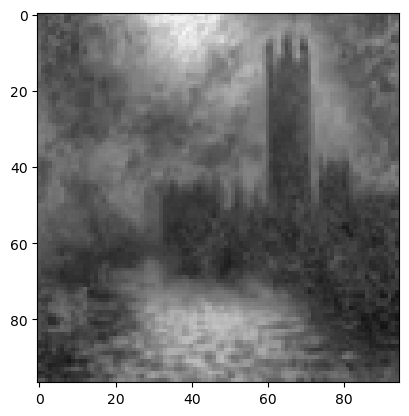
\includegraphics[width=0.5\textwidth]{./report/output1.png} %0.5指图片宽度
			
		\end{minipage}%
		\begin{minipage}[c]{0.2\textwidth}
			\centering
			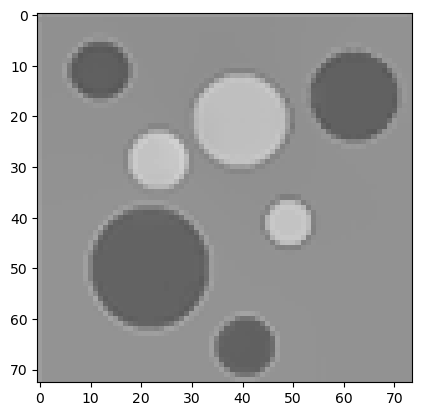
\includegraphics[width=0.7\textwidth]{./report/output2.png}
			
		\end{minipage}
		\begin{minipage}[c]{0.2\textwidth}
			\centering
			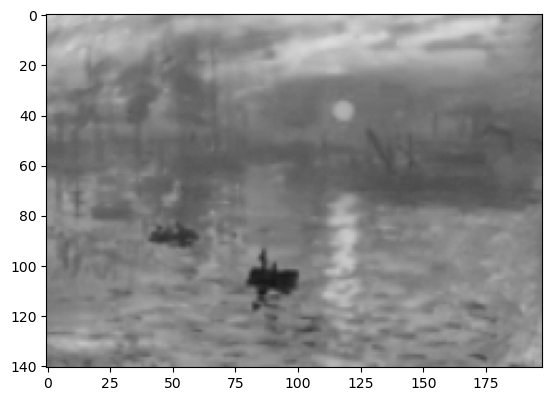
\includegraphics[width=0.8\textwidth]{./report/output3.png}
			
		\end{minipage}
		\caption*{改进方法结果}
%	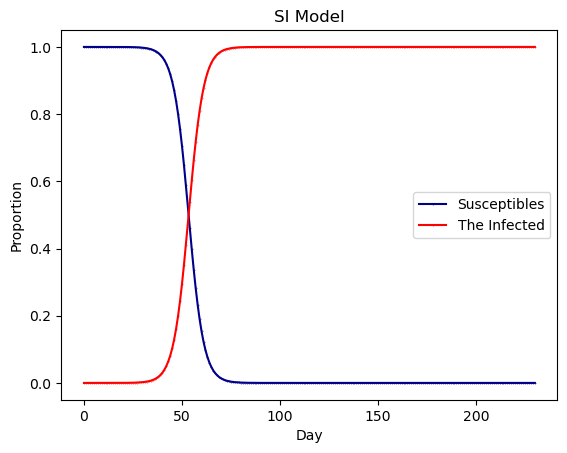
\includegraphics [width=0.2\textwidth]{1.png} \caption{渐变} %另起一行放图片
\end{figure}


\begin{figure}[htbp]
	\centering
		\begin{minipage}[c]{0.3\textwidth} %minipage使之保持同一行,0.2占这行的0.2
			\centering
			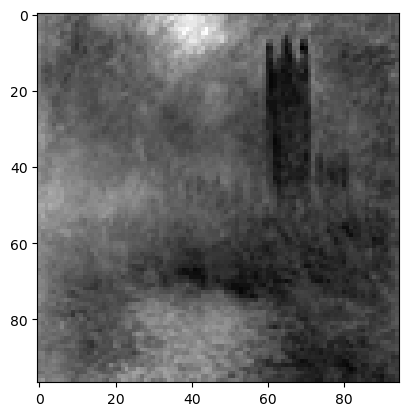
\includegraphics[width=0.5\textwidth]{./report/output4.png} %0.5指图片宽度
			
		\end{minipage}%
		\begin{minipage}[c]{0.2\textwidth}
			\centering
			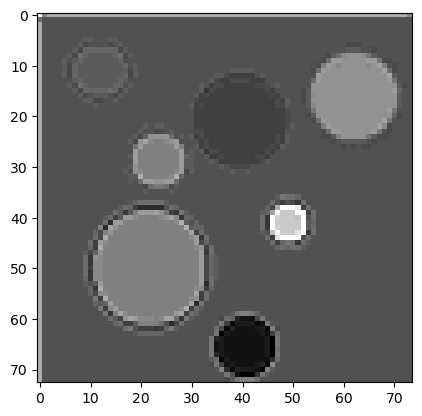
\includegraphics[width=0.7\textwidth]{./report/output5.png}
			
		\end{minipage}
		\begin{minipage}[c]{0.2\textwidth}
			\centering
			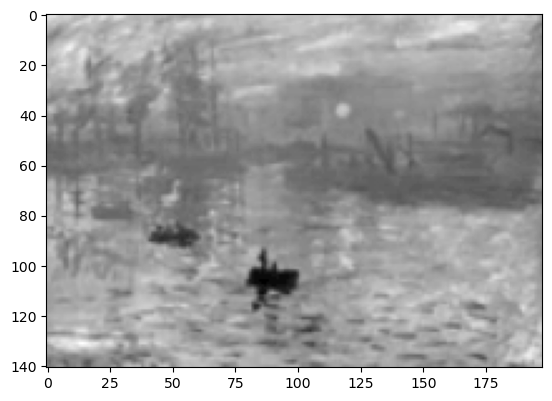
\includegraphics[width=0.8\textwidth]{./report/output6.png}
			
		\end{minipage}
		\caption*{使用OpenCV直接进行灰度读取结果}
%	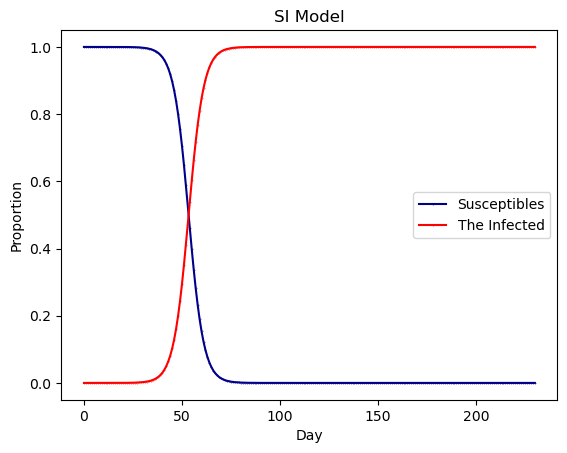
\includegraphics [width=0.2\textwidth]{1.png} \caption{渐变} %另起一行放图片
\end{figure}


\begin{figure}[htbp]
	\centering
		\begin{minipage}[c]{0.3\textwidth} %minipage使之保持同一行,0.2占这行的0.2
			\centering
			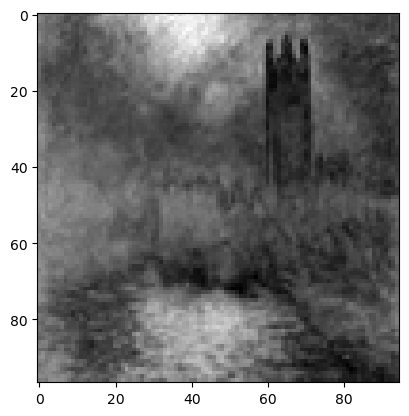
\includegraphics[width=0.5\textwidth]{./report/output7.png} %0.5指图片宽度
			
		\end{minipage}%
		\begin{minipage}[c]{0.2\textwidth}
			\centering
			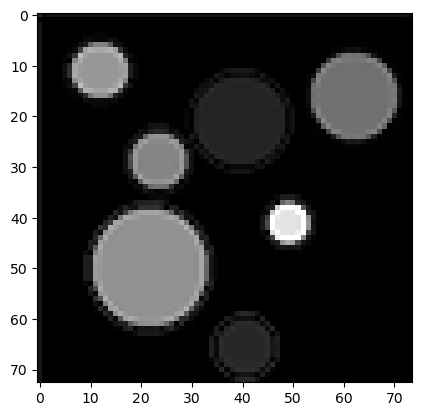
\includegraphics[width=0.7\textwidth]{./report/output8.png}
			
		\end{minipage}
		\begin{minipage}[c]{0.2\textwidth}
			\centering
			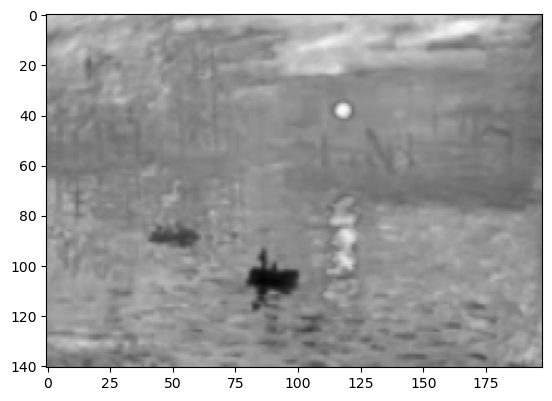
\includegraphics[width=0.8\textwidth]{./report/output9.png}
			
		\end{minipage}
		\caption*{使用最大值方法结果}
%	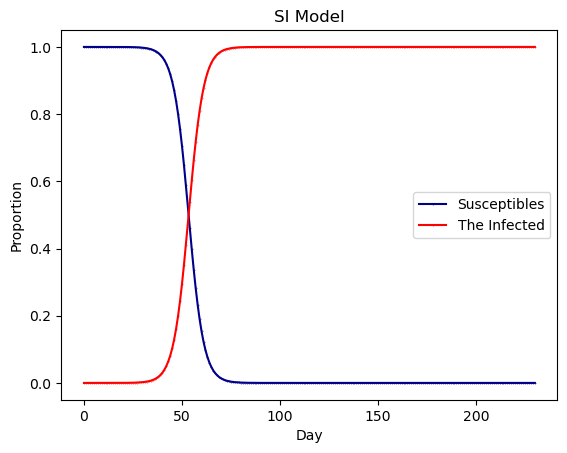
\includegraphics [width=0.2\textwidth]{1.png} \caption{渐变} %另起一行放图片
\end{figure}

\begin{figure}[htbp]
	\centering
		\begin{minipage}[c]{0.3\textwidth} %minipage使之保持同一行,0.2占这行的0.2
			\centering
			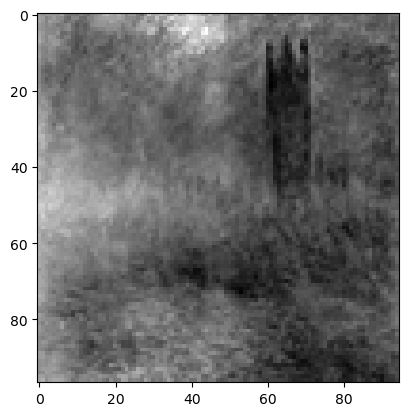
\includegraphics[width=0.5\textwidth]{./report/output11.png} %0.5指图片宽度
			
		\end{minipage}%
		\begin{minipage}[c]{0.2\textwidth}
			\centering
			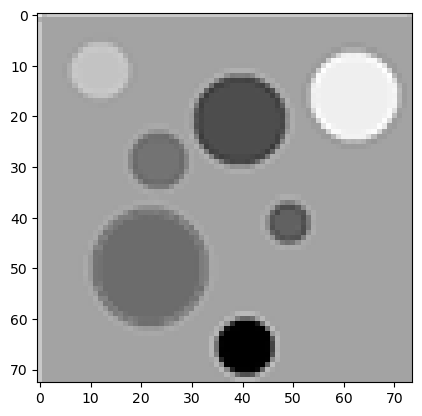
\includegraphics[width=0.7\textwidth]{./report/output12.png}
			
		\end{minipage}
		\begin{minipage}[c]{0.2\textwidth}
			\centering
			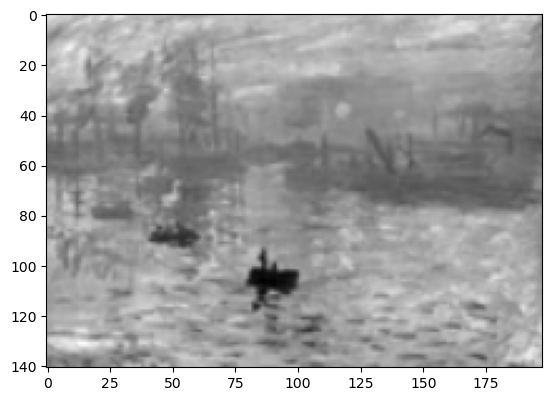
\includegraphics[width=0.8\textwidth]{./report/output13.png}
	
		\end{minipage}
		\caption*{使用均值法结果}
%	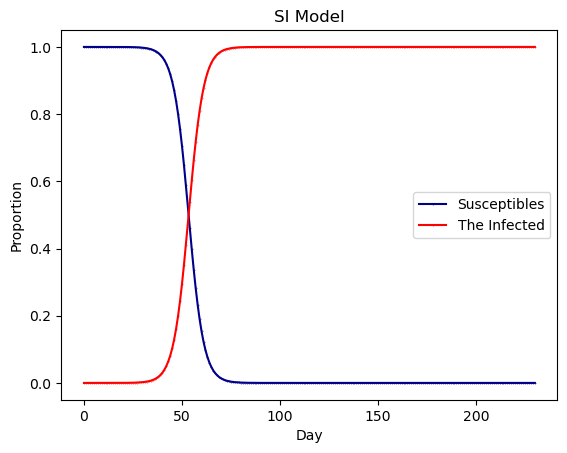
\includegraphics [width=0.2\textwidth]{1.png} \caption{渐变} %另起一行放图片
\end{figure}

\begin{figure}[htbp]
	\centering
		\begin{minipage}[c]{0.3\textwidth} %minipage使之保持同一行,0.2占这行的0.2
			\centering
			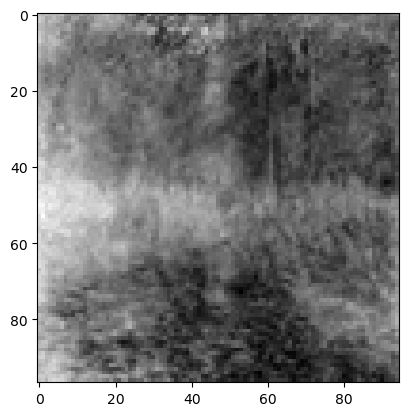
\includegraphics[width=0.5\textwidth]{./report/output14.png} %0.5指图片宽度
			
		\end{minipage}%
		\begin{minipage}[c]{0.2\textwidth}
			\centering
			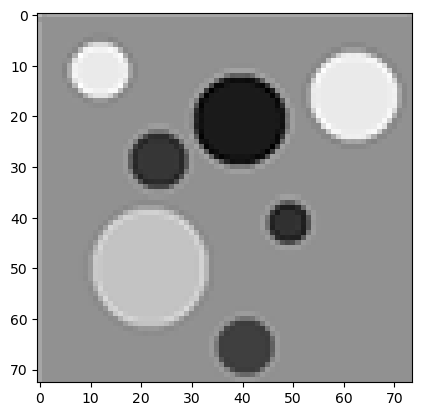
\includegraphics[width=0.7\textwidth]{./report/output15.png}
			
		\end{minipage}
		\begin{minipage}[c]{0.2\textwidth}
			\centering
			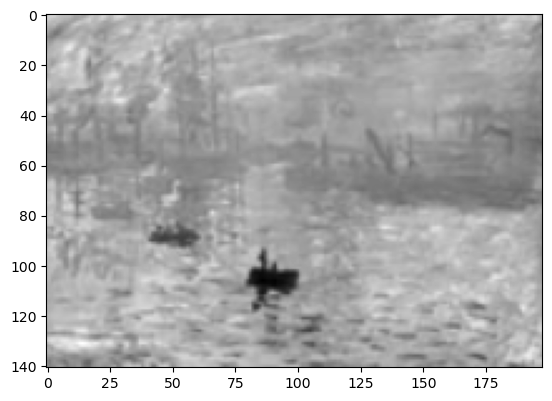
\includegraphics[width=0.8\textwidth]{./report/output16.png}
			
		\end{minipage}
		\caption*{使用加权平均法结果}
%	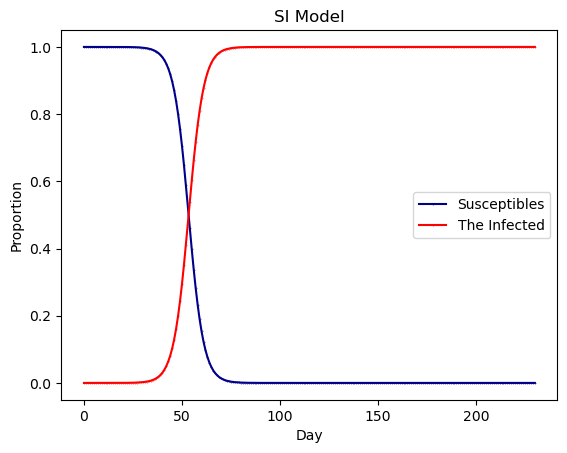
\includegraphics [width=0.2\textwidth]{1.png} \caption{渐变} %另起一行放图片
\end{figure}
 \setcounter{section}{8}
\section*{\centerline{八、结论}}
    从结果可知,改进后的方法可以更多的保留原彩色图像的显著特征。
    
    在将色差$ \vec{\Delta C_{ij}} $从二维降至一维的过程采用了主成分分析(PCA)的方法,
    即彩色图像灰度化并保留特征的过程实际上是一个通过最小二乘法进行数据降维的过程。

 \setcounter{section}{9}
\section*{\centerline{九、问题}}
    虽然改进后的算法可以极大程度的保留彩色图像的特征,但其理论时间复杂度达到了$O(m^{4})$ ,在处理高分辨率图像时,灰度化时间
    消耗过于庞大。




    

\bibliographystyle{plain}
\bibliography{refer}
\end{document}